\documentclass[10pt,twocolumn,letterpaper]{article}

\usepackage{cvpr}
\usepackage{times}
\usepackage{epsfig}
\usepackage{graphicx}
\usepackage{amsmath}
\usepackage{amssymb}
\usepackage{multirow}
\usepackage[utf8]{inputenc}
\usepackage{stfloats}
\usepackage{afterpage}

% Include other packages here, before hyperref.

% If you comment hyperref and then uncomment it, you should delete
% egpaper.aux before re-running latex.  (Or just hit 'q' on the first latex
% run, let it finish, and you should be clear).
\usepackage[breaklinks=true,bookmarks=false]{hyperref}

\cvprfinalcopy % *** Uncomment this line for the final submission

\def\cvprPaperID{****} % *** Enter the CVPR Paper ID here
\def\httilde{\mbox{\tt\raisebox{-.5ex}{\symbol{126}}}}

% Pages are numbered in submission mode, and unnumbered in camera-ready
%\ifcvprfinal\pagestyle{empty}\fi
\setcounter{page}{1}
\begin{document}

%%%%%%%%% TITLE
\title{Ensembled Transfer Learning for MRI-based Knee Injury Diagnosis}

\author{Shayne Miel\\
Stanford University\\
Stanford, CA, USA\\
{\tt\small smiel@stanford.edu}
% % For a paper whose authors are all at the same institution,
% % omit the following lines up until the closing ``}''.
% % Additional authors and addresses can be added with ``\and'',
% % just like the second author.
% % To save space, use either the email address or home page, not both
% \and
% Second Author\\
% Institution2\\
% First line of institution2 address\\
% {\tt\small secondauthor@i2.org}
}

\maketitle
%\thispagestyle{empty}

%%%%%%%% ABSTRACT
\begin{abstract}
   Improving the accuracy with which automated methods can identify injuries in
   MRIs of the knee would lead to time and cost savings for doctors and patients.
   I show that by ensembling a collection of transfer learning models that use pretrained neural networks for feature extraction, as well as a mixture of max pooling and an attention mechanisms to combine features from multiple
   frames of the MRI scan, I can improve upon the current state of the art on
   the MRNet data set.
\end{abstract}

%%%%%%%%% BODY TEXT
\section{Introduction} % (0.5-1 page)
% Explain the problem and why it is important. Discuss your motivation for pursuing this problem. Give some background if necessary. Clearly state what the input and output is. Be very explicit: "The input to our algorithm is a {image, video, patient age, 3D video, etc.}. We then use a {SVM, CNN, GAN, etc.} to output a predicted {age, cancer type, restaurant, ramen, etc.}." This is very important since different teams have different inputs/outputs spanning different application domains. Being explicit about this makes it easier for readers.

Magnetic resonance imaging (MRI) is a method of obtaining three dimensional images of the inside of an object by using strong magnets to align the protons in the object and then radio frequency currents to disrupt and measure that alignment. An MRI sequence is a series of two dimensional images that can be stacked to recreate the three dimensional object. There are three sequence types, each corresponding to an orientation of the ``camera'' that captures the two dimensional slices. The axial sequence captures slices of the object that are horizontal to the ground; the coronal sequence captures vertical slices as viewed from the front of the object; and the sagittal sequence captures vertical slices as viewed from the side of the object.

MRI can be a useful tool when diagnosing knee injuries\cite{orlando2015diagnosis,figueiredo2018use,smith2012diagnostic}, however, analyzing the images is a time-consuming process and even with trained professionals, it is easy for a clinician to misdiagnose an injury based on an MRI reading\cite{kolata2011}. Improving the automated identification of abnormalities in knee MRIs could help prioritize which MRIs to examine first, as well as provide better early results for patients whose scans appear normal. Model predictions could also provide a ``second opinion'' which would reduce the possibility of missed abnormalities. This could represent a large cost savings for hospitals and an increased level of care for patients.

The problem addressed in this paper is as follows: given a set of three MRI sequences (axial, coronal, and sagittal) of a patient's knee, can we predict the presence of injuries that will require surgery? In particular, we wish to predict whether the knee is healthy, has an ACL tear, has a meniscal tear, or has any other abnormality. Since these injuries can co-occur, we wish to predict three independent binary values: abnormal, acl tear, and meniscus tear. Past research has proven that MRI scans are accurate and sensitive tools for detecting these kinds of injuries in a non-invasive manner\cite{boeve1991magnetic,felli2016comparison,yaqoob2015diagnostic}.


\section{Related work}
\label{related-work} % (0.5-1 page)
% You should find existing papers, group them into categories based on their approaches, and talk about exemplary ones in each category: Discuss strengths and weaknesses. In your opinion, which approaches were clever/good? What is the state-of-the-art? Do most people perform the task by hand? You should aim to have at least 10 references in the related work. Include previous attempts by others at your problem, previous technical methods, or previous learning algorithms. Google Scholar is very useful for this: https://scholar.google.com/ (you can click “cite” and it generates MLA, APA, BibTeX, etc.) You can also try http://www.arxiv-sanity.com/ to search for recent arXiv papers.

There are two main challenges when trying to use automated methods on MRI sequences. The first is that each MRI image has high information content because it is a 3-dimensional image of the patient. Determining how to extract meaning from a variable length series of images is not trivial. By contrast, the second challenge is that MRIs are difficult and expensive to collect, which means that MRI data sets are too small for most deep learning approaches. This means that deep learning models must be constrained to a limited number of updates to prevent overfitting.

Most recent deep learning MRI work deals with the 3-dimensional nature of MRI images by using 3D-CNNs, which take the idea of $(channel, width, height)$ convolutions that are swept across a 2-dimensional image and extends them to $(time, channel, width, height)$ convolutions that are swept across the 3-dimensional image
\cite{hosseini2016alzheimer,wei2018flair,khvostikov20183d,zou20173d}. These models are limited, however, by the number of parameters required for 3D-CNNs and the need to train them from scratch.

Another common method is the so-called 2.5D approach, where models are trained on sliding windows of the input sequence \cite{roth2015improving,alkadi20182,grovik2019deep}. This works well for sequence-to-sequence problems, but doesn't help when you need to reduce the MRI to a single prediction.

RNNs provide yet another avenue for processing a series of 2-D images, as done in \cite{qin2019convolutional,han2018mri}. However, the need to train from scratch and the number of parameters in these kinds of models still presents a very real challenge for small data sets.

The closest model to the ones in this paper is Bien et al.'s MRNet\cite{bien2018deep}, which is the current state-of-the-art MRNet for diagnosing injuries in MRI scans of the knee. Their method uses conventional convolutional neural networks, which allows them to jump start the training process by pretraining an AlexNet\cite{krizhevsky2012imagenet} network on a large data set like ImageNet\cite{imagenet_cvpr09}. The sequence of images are each fed through the pretrained network to generate an $(s \times c \times w \times h)$ tensor, where $s$ is the sequence length, $c$ is the channel depth, $w$ is the width and $h$ is the height. The width and height dimensions are reduced via global average pooling\cite{lin2013network}, so that they are left with an $(s \times c)$ tensor. Those features are then reduced via max pooling over the sequence and fed through a linear classifier and sigmoid activation to predict a probability for the sequence. Three sequence-level probabilities (axial, coronal, and sagittal) are then sent to a logistic regression classifier to obtain a final diagnosis probability.

\begin{figure*}
\begin{center}
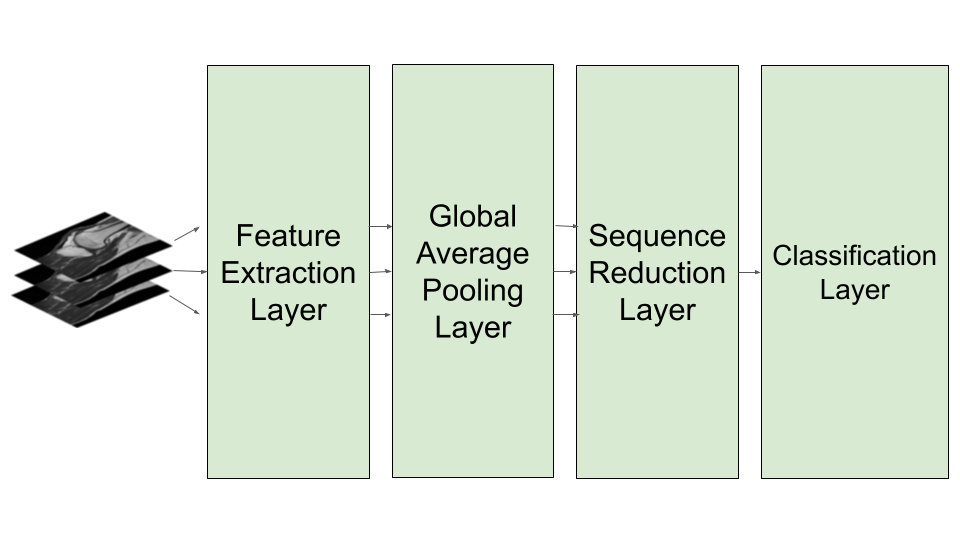
\includegraphics[width=0.6\linewidth]{../images/diagram/network2.png}
\end{center}
   \caption{An abstract view of the sequence-specific networks. Image of a knee MRI taken from \cite{knee-image}.}
\label{fig:network}
\end{figure*}

\section{Methods} % (2 pages)
% Describe your learning algorithms, proposed algorithm(s), or theoretical proof(s). Make sure to include relevant mathematical notation. For example, say what the softmax function is or include your loss equation. It is okay to use formulas from the lecture notes. For each algorithm, give a brief description (2-3 sentences) of how it works. Again, we are looking for your understanding of how these deep learning algorithms work. Although the teaching staff probably know the algorithms, future readers may not (reports will be posted on the class website). Additionally, if you are using a niche or cutting-edge algorithm (e.g. binary network, SURF features, or anything else not covered in the class), you may want to explain your algorithm using several paragraphs. Note: Theory/algorithms projects may have an appendix showing extended proofs (see appendix description below). Assume the reader has completed CS 231N. You don't need to explain filters and max-pooling, but if you do something like stochastic strides, then you should explain that.

% My goals for this project are fairly simple:
% \begin{enumerate}
%    \item Reproduce the results obtained by Bien, et al. in \cite{bien2018deep}.
%    \item Experiment with using different pretrained networks to extract features,
%    specifically replacing AlexNet with GoogLeNet \cite{szegedy2015going} as Chi, et al. did for ultrasound images \cite{chi2017thyroid}, ResNet \cite{he2016deep} as done in \cite{korfiatis2017residual}, and Inception-v3 \cite{szegedy2016rethinking} as done in \cite{kim2018artificial}.
%    \item If time allows, try replacing the logistic regression ensemble with a direct concatenation of the features from each of the three series before going through the fully connected layer.
% \end{enumerate}

\subsection{Sequence Network}

Figure \ref{fig:network} shows an abstract process for turning a single MRI sequence into an injury prediction. On the left side of the diagram, a series of $n$ images, each a $\mathbb{R}^{3 \times 224 \times 224}$ matrix, are fed into the network as a single batch. The feature extractor converts each of these images into a $\mathbb{R}^{c \times w \times h}$ matrix, where $c$ is the number of channels and $w$ and $h$ are the width and height, respectively. These features are then flattened into a series of $\mathbb{R}^c$ vectors in the global average pooling layer. Finally, the full batch of $n$ vectors are flattened into a single $\mathbb{R}^c$ vector in the sequence reduction layer. This vector is then passed through a linear layer and a sigmoid activation in the classification layer to arrive at a probability for whether the entire MRI sequence indicates the injury in question.

Concretely, if we describe the feature extraction layer as a function, $f: \mathbb{R}^{n \times 3 \times 244 \times 244} \rightarrow \mathbb{R}^{n \times c \times w \times h}$, and the sequence reduction layer as a function $g: \mathbb{R}^{n \times c} \rightarrow \mathbb{R}^c$, then the entire network can be written as:

$$ gap_{jk}(x) = \frac{\sum_{i=1}^n x_{j,k}^{(i)}}{n} $$

\begin{equation}
\label{eq:network}
p = \sigma(g(gap(f(x))) W_c + b_c)
\end{equation}

where $p$ is the predicted probability, $W_c \in \mathbb{R}^{c \times 1}$ and $b_c \in \mathbb{R}^c$ are the weights and biases of the classification layer and $\sigma$ is the sigmoid function: $\frac{1}{1 + e^{-x}}$

The current state-of-the-art system, MRNet - which was discussed in detail in Section \ref{related-work}, can be described as using parts of a pretrained AlexNet for the feature extractor layer, and an element-wise maximum to flatten the sequence in the sequence reduction layer.

\subsection{SqueezeNet}


\begin{figure}
\begin{center}
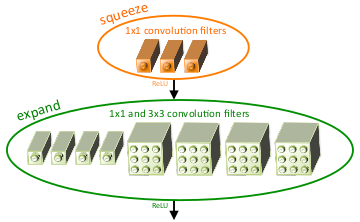
\includegraphics[width=0.6\linewidth]{../images/fire/fire.png}
\end{center}
   \caption{Illustration of a fire layer. Taken directly from ``SqueezeNet: AlexNet-level accuracy with 50x fewer parameters and $<$0.5 MB model size''\cite{iandola2016squeezenet}}
\label{fig:fire}
\end{figure}

SqueezeNet is a deep convolutional neural network that achieves high performance on the ImageNet challenge. It is composed of a series of ``fire'' layers, each of which consists of a layer of $1 \times 1$ convolutional filters (the squeeze layer), followed by a ReLU and then a mix of $1 \times 1$ and $3 \times 3$ convolutional layers (the expand layer) whose outputs are concatenated before going through a final ReLU activation. An illustration of a fire layer is shown in Figure \ref{fig:fire}. These layers are interspersed with max pooling layers before the 1st, 4th, and 8th fire layers, and the entire network begins with a traditional $7 \times 7$ convolutional layer.

Fine-tuning a SqueezeNet model that has been pretrained on the ImageNet data set is a method that has been used successfully to classify vehicles\cite{agoes2017fine}, crop disease\cite{durmucs2017disease}, and cataracts\cite{qian2018machine}. By removing the final dropout, convolution, ReLU and adaptive average pooling layers from the pretrained network, we can use it as a drop-in replacement for the feature extraction layer in Figure \ref{fig:network}.

\subsection{Attention}
Attention is a mechanism that has traditionally been applied as a summarization method of the hidden states in a recurrent neural network. Given some query $\textbf{Q}$, a set of keys $\textbf{K}$, and a set of values $\textbf{V}$, the attention score can be calculated as

$$s = (\textbf{Q}\textbf{K}^T)\textbf{V}$$
$$\textbf{A}_i = \frac{e^{s_i}}{\sum_{j=1}^k e^{s_j}}$$
 as described by Tan, et al.\cite{tan2018deep}, whose work was derived from Luong et. al's location-based attention\cite{luong2015effective}.

In the case of an RNN, the query is often the final hidden state, the keys are either the input embeddings or the hidden states at each time step, and the values are the hidden states at each time step. A final representation of the entire sequence can then be generated by taking the weighted sum of the values times the attention vector, $result = \textbf{A} \textbf{V}^T$.

For the experiments in this paper, we eschew the use of an RNN and simply use the attention-weighted sum across frames of the MRI sequence to generate the final representation of the sequence. In this case, the query is a learned parameter of the network, while the keys and values are both the output of the global average pooling layer for each frame in the sequence. This allows us to use the attention-weighted sum as the sequence-reduction layer:

$$ g(x) = \textbf{A} x^T$$

Because of the imbalanced class sizes, we train all of the sequence-specific models with a weighted binary cross-entropy loss:

$$ L = -\frac{1}{N} \sum_{i=0}^N w_i \big(y_i log(p_i) + (1 - y_i) log(1 - p_i)\big)$$

where $w_i$ is the fraction of the instances in the data set that have label $y_i$, and $p_i$ is the output of the network described by Equation \ref{eq:network} for sequence $i$.

\subsection{Sequence Ensembling}


\begin{figure}
\begin{center}
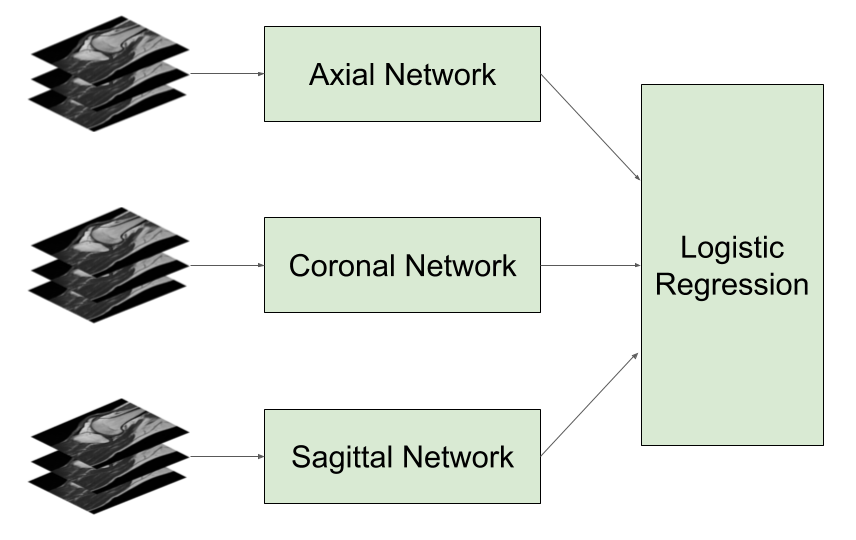
\includegraphics[width=0.8\linewidth]{../images/diagram/ensemble.png}
\end{center}
   \caption{Ensembling predictions from the sequence-specific networks to generate an injury prediction.}
\label{fig:ensemble}
\end{figure}

Because we have access to multiple MRI sequences per patient, separate networks can be trained for each of the axial, coronal, and sagittal sequences. The three probabilities are then fed into a logistic regression classifier to arrive at a final injury prediction, as shown in Figure \ref{fig:ensemble}.

\subsection{Model and Sequence Ensembling}
\begin{figure}
\begin{center}
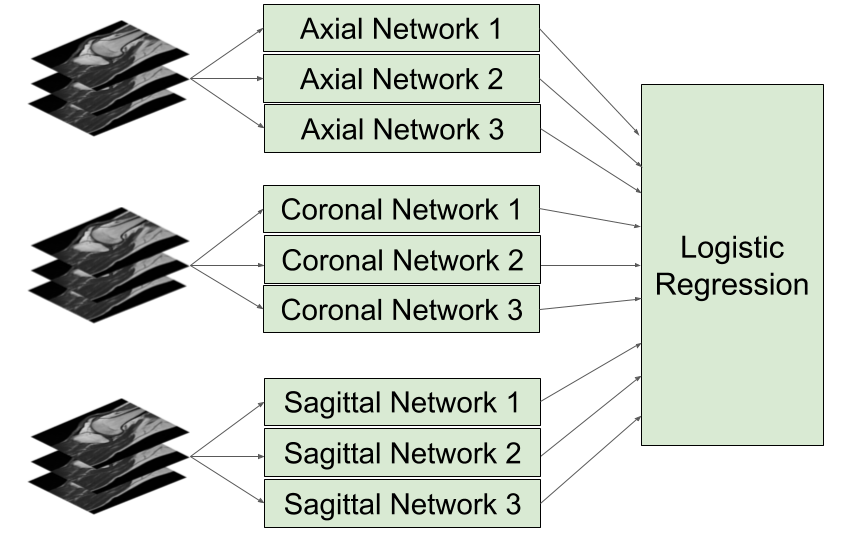
\includegraphics[width=0.8\linewidth]{../images/diagram/ensemble-of-ensembles.png}
\end{center}
   \caption{Ensembling predictions from multiple sequence-specific network types to generate an injury prediction.}
\label{fig:ensemble-of-ensembles}
\end{figure}

In addition to this per-model sequence ensembling, we can also use the sequence predictions from \textit{multiple model types} as features for a logistic regression model, as shown in Figure \ref{fig:ensemble-of-ensembles}, as a meta-ensemble.

\section{Dataset} % (0.5-1 pages)
% Give details about your dataset: how many training/validation/test examples do you have? Is there any preprocessing you did? What about normalization or data augmentation? What is the resolution of your images? How is your time-series data discretized? Include a citation to where you got your dataset from. Depending on available space, show some examples from your dataset. You should also talk about the features you used. If you extracted features using Fourier transforms, word2vec, histogram of oriented gradients (HOG), PCA, ICA, etc. make sure to talk about it. Try to include examples of your data in the report (e.g. include an image, show a waveform, price graph, etc.).

The MRI data provided in the \href{https://stanfordmlgroup.github.io/competitions/mrnet/}{MRNet challenge} contains scans from 3 MRI types (axial, coronal, and sagittal) with 3 labels per MRI (abnormality, ACL tear, and meniscal tear) for 1,250 examinations.

The released data has already been split into a training and validation set, and a test set has been withheld for leaderboard purposes. In order to evaluate my methods for this paper, I have further divided the training set into training and tuning sets, and am using the validation set for all reported metrics. Counts of cases and labels for each set can be seen in Table \ref{tab:dataset}.

\subsection{Preprocessing}

The data is provided as a collection of numpy\cite{numpy} 3-dimensional matrices, one per sequence per case. They have already been extracted from the Digital Imaging and Communications in Medicine (DICOM) files and scaled to $256 \times 256$ images.

During training, we crop the images to $224 \times 224$ to match the expected input size for a pretrained ImageNet model. We then standardize each input sequence by subtracting the minimum pixel value and dividing by the range observed in the sequence, then rescale the image to a $0-256$ range of pixel values. Finally, we normalize the sequence by subtracting the data set mean ($58.09$) and dividing by the data set standard deviation ($49.73$).

\subsection{Augmentation}

In order to prevent overfitting the small data set, we perform data augmentation during training. Every image is randomly flipped horizontally, shifted horizontally by -25 to 25 pixels, and rotated by -25 to 25 degrees each time it is seen during training. Note that the same transformation is applied to every image in a given sequence.

\begin{table}
\begin{center}
\begin{tabular}{|lc|c|c|c|}
\hline
Diagnosis & Label & Training & Tuning & Validation \\
\hline
\multirow{ 3}{*}{Abnormal} & Positive & 835 & 78 & 95 \\
                           & Negative & 175 & 42 & 25 \\
                           & Total & 1010 & 120 & 120 \\
\hline
\multirow{ 3}{*}{ACL}      & Positive & 167 & 41 & 54 \\
                           & Negative & 843 & 79 & 66 \\
                           & Total & 1010 & 120 & 120 \\
\hline
\multirow{ 3}{*}{Meniscus} & Positive & 353 & 44 & 52 \\
                           & Negative & 657 & 76 & 68 \\
                           & Total & 1010 & 120 & 120 \\
\hline
\end{tabular}
\end{center}
\caption{MRNet data splits and label counts.}
\label{tab:dataset}
\end{table}

\section{Results} % (2-3 pages)
% You should also briefly give details about what hyperparameters you chose (e.g. why did you use X learning rate for gradient descent or did you use Adam, what was your mini-batch size and why) and how you chose them. Did you do cross-validation, if so, how many folds? This should not take more than 1-2 paragraphs. If you want to list more details, please do so in the supplemental material.

% Before you list your results, make sure to list and explain what your primary metrics are: accuracy, mAP, inception/mode scores, etc. Provide equations for the metrics if necessary. For results, you want to have a mixture of tables and plots. If you are solving a classification problem, you should include a confusion matrix or AUC/AUPRC curves. Include performance metrics such as precision, recall, and accuracy. For regression problems, state the at least the average error. For reinforcement learning and control, have appropriate metrics as well.

% You should have both quantitative and qualitative results. To reiterate, you must have both quantitative and qualitative results! This includes unsupervised learning (talk with the TAs on how to quantify unsupervised methods). Include visualizations of results, heatmaps, saliency maps, examples of where your algorithm failed and a discussion of why certain algorithms failed or succeeded. In addition, explain whether you think you have overfitted to your training set and what, if anything, you did to mitigate that. Make sure to discuss the figures/tables in your main text throughout this section. Your plots should include legends, axis labels, and have font sizes that are readable when printed.

% Here’s a list of qualitative & quantitative methods for analysis that might be helpful in your project. None of these are necessary nor will be explicitly looked for by graders – rather, we wanted to provide guidance on analysis methods:

% Saliency maps

% Class visualization

% t-SNE

% Confusion matrices

% Common qualitative errors

% GANs: compare the generated output to NN in training set (quant and qualitative)

% GANs: image quality metrics like Inception and Mode scores

% VAE: Reporting measures like Annealed Importance Sampling (AIS)
\begin{table*}
\begin{center}
\begin{tabular}{|l|c|c|}
\hline
Name & Feature Extraction Layer & Sequence Reduction Layer \\
\hline
MRNet & AlexNet & Max pooling \\
MRNet-Squeeze & SqueezeNet & Max pooling \\
MRNet-Attend & AlexNet & Attention \\
MRNet-SqueezeAttend & SqueezeNet & Attention \\
\hline
\end{tabular}
\end{center}
\caption{Model combinations used in experiments.}
\label{tab:models}
\end{table*}

Referring to the abstract network image shown in Figure \ref{fig:network}, Table \ref{tab:models} shows the combinations of feature extraction and sequence reduction techniques used in the experiments in this paper. In each case, a pretrained network that was tuned on ImageNet was used to extract features. The pretrained network was fine-tuned on the MRNet data along with the other layers of the model.

In addition to these models, I include results from ensembling the sequence-specific predictions of all four models, as described in Figure \ref{fig:ensemble-of-ensembles}.

\begin{table}
\begin{center}
\begin{tabular}{|l|l|}
\hline
Optimization Method & Adam \\
Weight Decay & 0.01 \\
\hline
Learning Rate Schedule & Reduce on plateau \\
Initial Learning Rate & 0.00001 \\
Max Patience & 5 \\
Factor & 0.3 \\
\hline
Max Epochs & 40 \\
\hline
Logistic Regression Penalty & L2 \\
Logistic Regression Lambda & 1.0 \\
\hline

\end{tabular}
\end{center}
\caption{Hyperparameters for all experiments.}
\label{tab:hyperparams}
\end{table}

Table \ref{tab:hyperparams} shows the hyperparameters used for all experiments. Most of these hyperparameters were drawn from the original MRNet paper, although Initial Learning Rate and Max Epochs were determined with brief experiments on the axial sequence and abnormal label. Due to the processing time required to run these models, extensive hyperparameter optimization was not feasible, although this would be a potential are for future work.

The primary metric used to compare models is Area Under the ROC Curve (AUC). In particular, averaging the AUC of the three labels determines a final metric for each model. In addition, I report the specificity, sensitivity, and accuracy of the four models on each label, using a $0.5$ threshold to turn probabilities into label predictions.

Table \ref{tab:results} shows the AUC for each model on each injury prediction, as well as averaged across all injuries. Each of the individual model types perform well on some of the injury categories, but none of them excel at all injuries. For detecting any kind of abnormality, the original MRNet implementation gets the highest AUC $(0.940)$. MRNet-Squeeze is the best model for detecting ACL injuries $(0.974)$, while MRNet-SqueezeAttend achieves the highest AUC on the Meniscal tear category $(0.885)$.

By using all four model types together, however, I can capture that varying performance on the three injuries to create an ensembled model that outperforms any of the individual models. The ensembled model achieves nearly the highest AUC on all individual injury types, and significantly outperforms the others with an average AUC of $0.931$.

MRNet (reported) is the AUC reported by Bien, et al.\cite{bien2018deep}, and is not directly comparable to the values shown here because the released data is a subset of the data used in their experiments.

\begin{table*}[h!]
\begin{center}
\begin{tabular}{|l|c|c|c|c|}
\hline
Model & Average & Abnormal & ACL & Meniscus \\
\hline
MRNet (reported) & 0.916 & 0.937 & 0.965 & 0.847 \\
\hline
MRNet & 0.913 & \textbf{0.940} & 0.960 & 0.839 \\
MRNet-Squeeze & 0.910 & 0.925 & 0.974 & 0.829 \\
MRNet-Attend & 0.891 & 0.925 & 0.910 & 0.838 \\
MRNet-SqueezeAttend & 0.915 & 0.936 & 0.925 & \textbf{0.885}\\
\hline
Ensemble & \textbf{0.931} & 0.939 & \textbf{0.976} & 0.876 \\
\hline
\end{tabular}
\end{center}
\caption{AUC on the validation set}
\label{tab:results}
\end{table*}

Table \ref{tab:metrics} shows the specificity, sensitivity, and accuracy of each model, as well as the human performance of expert radiologists, as reported by Bien et al.\cite{bien2018deep}. Once again, the experiments in this paper are not directly comparable to the reported human values because of differing data sets, especially on these metrics since class imbalance can have an outsized effect on precision and recall. On these metrics, the final ensemble achieves state of the art on some injury types and not others.

\begin{table*}[h!]
\begin{center}
\begin{tabular}{|l|c|c|c|}
\hline
Prediction & Specificity & Sensitivity & Accuracy \\
\hline
\multicolumn{4}{l}{\textbf{Abnormality} }\\
\hline
Radiologist & 0.844 & 0.905 & 0.894 \\
MRNet (reported) & 0.714 & 0.879 & 0.850 \\
\hline
MRNet & 0.440 & 0.968 & 0.858 \\
MRNet-Squeeze & 0.560 & 0.968 & 0.883 \\
MRNet-Attend & 0.480 & 0.979 & 0.875  \\
MRNet-SqueezeAttend & 0.440 & 0.968 & 0.858 \\
\hline
Ensemble & 0.480 & 0.958 & 0.858 \\
\hline
\multicolumn{4}{l}{\textbf{ACL tear} }\\
\hline
Radiologist & 0.933 & 0.906 & 0.920 \\
MRNet (reported) & 0.968 & 0.759 & 0.867 \\
\hline
MRNet & 0.894 & 0.907 & 0.900 \\
MRNet-Squeeze & 0.909 & 0.963 & 0.933 \\
MRNet-Attend & 0.803 & 0.778 &  0.792 \\
MRNet-SqueezeAttend & 0.864 & 0.852 & 0.858 \\
\hline
Ensemble & 0.909 & 0.981 & 0.942 \\
\hline
\multicolumn{4}{l}{\textbf{Meniscus tear} }\\
\hline
Radiologist & 0.882 & 0.820 & 0.849 \\
MRNet (reported) & 0.741 & 0.710 & 0.725 \\
\hline
MRNet & 0.721 & 0.788 & 0.750 \\
MRNet-Squeeze & 0.735 & 0.731 & 0.733 \\
MRNet-Attend & 0.691 & 0.846 &  0.758 \\
MRNet-SqueezeAttend & 0.794 & 0.750 & 0.775 \\

\hline
Ensemble & 0.735 & 0.865 & 0.792 \\
\hline
\end{tabular}
\end{center}
\caption{Metrics on the validation set}
\label{tab:metrics}
\end{table*}

\begin{figure*}[h!]
\begin{center}
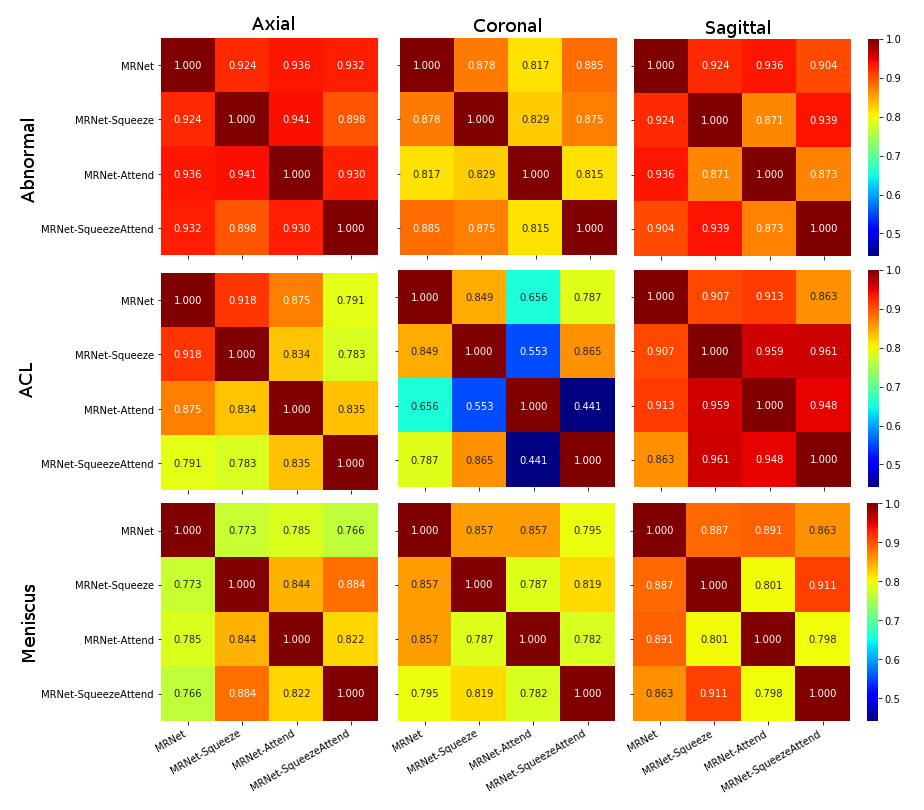
\includegraphics[width=0.9\linewidth]{../images/corr2/corr2.png}
\end{center}
   \caption{Correlation between sequence-specific predictions on the validation set.}
\label{fig:corr}
\end{figure*}



It is interesting to consider the differences between the four models, especially at the level of the sequence-specific predictions (i.e. the values that get fed into the logistic regression classifier). If the sequence-specific predictions for each diagnosis are highly correlated, then we would not expect the multi-model ensemble to outperform the individual models. Figure \ref{fig:corr} shows the correlation between the sequence-specific predictions on the validation set for the four models. There is a strong correlation between the sequence-specific predictions on some diagnosis/sequence combinations (for instance, Abnormal/Axial and ACL/Sagittal), but on other combinations the correlation is quite low (ACL/Coronal, Meniscus/Axial). These areas of low correlation are likely useful signals for the multi-model ensemble.

\begin{table}[h!]
\begin{center}
\begin{tabular}{|l|l|}
\hline
Model & Frame \\
\hline
MRNet & 11 \\
MRNet-Squeeze & 7 \\
MRNet-Attend & 20 \\
MRNet-SqueezeAttend & 6 \\
\hline
\end{tabular}
\end{center}
\caption{The most focused on frame of the axial sequence for each model when predicting whether Case 1218 has an ACL tear.}
\label{tab:frames}
\end{table}

Another way to look at the differences between models is to examine, for a particular diagnosis/sequence combination, what areas of the MRI each model is focusing on. If we consider a specific instance in the validation set, Case 1218, and look at a specific diagnosis/sequence pair, ACL/Axial, we can ask which image from the sequence each model is most interested in. For the models that use attention (MRNet-Attend and MRNet-SqueezeAttend) that simply means asking for the argmax of the calculated attention vector. For MRNet and MRNet-Squeeze, the sequence reduction layer takes the maximum value over the sequence for each location in the features vector. For those models, we can say that the frame with the most maximum values is the one that the model is ``most interested'' in. Table \ref{tab:frames} shows the most interesting frame of the axial sequence for each model when asked to predict whether Case 1218 has an ACL tear.

We can go further though, and examine the class activation map (CAM) for each of those frames for each model. A class activation map is a way of visualizing where in the image a model is focusing its (implicit) attention\cite{zhou2016learning}. To calculate the CAM for the frames listed in Table \ref{tab:frames}, we use $W_c$ from Equation \ref{eq:network} to compute a weighted average of the $c$ $\mathbb{R}^{w \times h}$ feature maps generated by running the single frame through the feature extraction layer of the sequence-specific model. That is, let $F$ be the $\mathbb{R}^{c \times w \times h}$ tensor returned by running a frame through the feature extraction layer. Then we calculate an image $I \in \mathbb{R}^{w \times h}$:

$$I_{i,j} = \frac{1}{c} \sum_{a=1}^c W_{c_a} F_{i, j}$$

By scaling this image up to the original MRI image size $(256 \times 256)$ and using the values as a colormap to overlay on the image, we can create a visualization of where the model's attention is focused for each frame. Figure \ref{fig:cam_4x4} shows the CAM for the four models (across the columns) for the 11th, 7th, 20th, and 6th frame, i.e. each model's ``most interesting'' frame (across the rows).

\begin{figure*}[h!]
\begin{center}
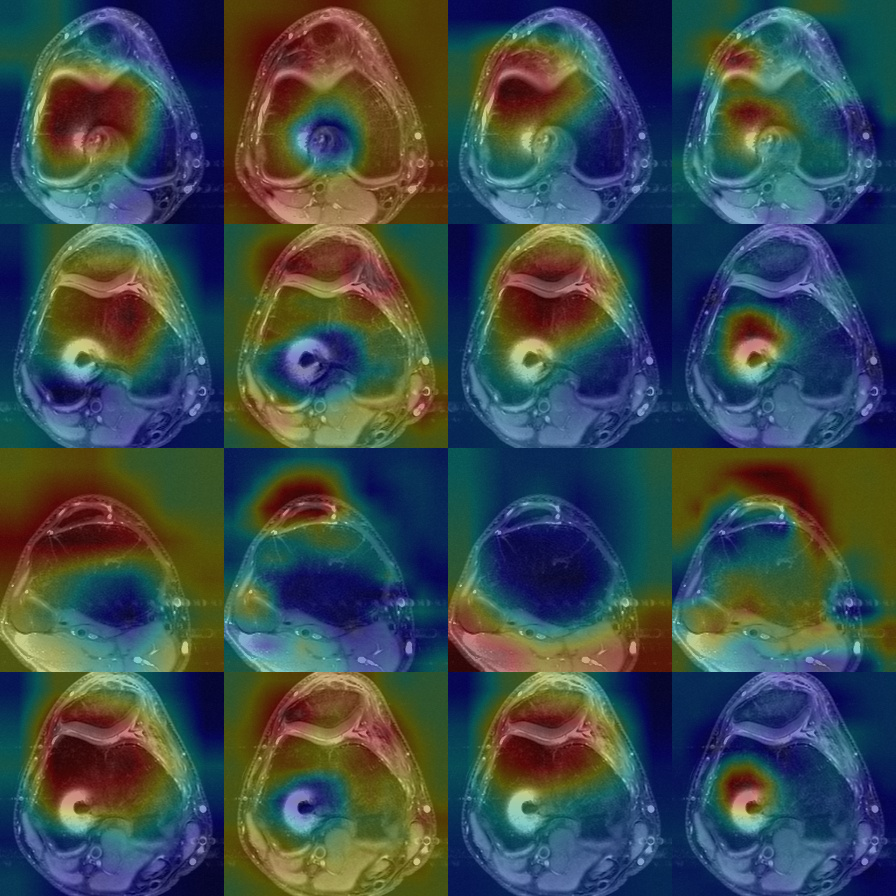
\includegraphics[width=0.9\linewidth]{../images/cams/4x4.png}
\end{center}
   \caption{Class activation maps from the four networks for the axial sequence of Case 1218, when asked to predict whether there is an ACL tear. From left to right, the columns are class activation maps for MRNet, MRNet-Squeeze, MRNet-Attend, and MRNet-SqueezeAttend. Each row represents the frame from the axial sequence that each network found most interesting.}
\label{fig:cam_4x4}
\end{figure*}


\section{Conclusion/Future Work} % (1-3 paragraphs)
% Summarize your report and reiterate key points. Which algorithms were the highest-performing?  Why do you think that some algorithms worked better than others? For future work, if you had more time, more team members, or more compute, what would you explore?

The experiments in this paper use transfer learning to predict injury diagnoses from MRI sequences of the knee. I compare pretrained AlexNet and SqueezeNet models as feature extractors and max pooling versus attention mechanisms to reduce the information across the sequence. Finally, I use a logistic regression, trained on the sequence-specific predictions, to predict the probability of the diagnosis for the patient.

I show that all of the models have different strengths and weaknesses, some achieving higher AUC scores than others on each diagnosis. Furthermore, I show that by ensembling not just different sequence predictions, but multiple sequence predictions from multiple sequence models, I can outperform the current state of the art on the MRNet data set.

There is still a lot left to explore here though. Future work should include examining how to get greater diversity in the sequence-specific models. Some possibilities for decreasing the correlation between predictions are:
\begin{itemize}
\item Using other pretrained feature extractors in the Feature Extraction layer.
\item Swapping the order of the Global Average Pooling layer and the Sequence
Reduction layer.
\item Using more advanced methods like RNNs in the Sequence Reduction layer.
\end{itemize}

I also believe that there is a possibility of using inter-sequence attention to compute a final representation of all three sequences, but exploring that was beyond the scope of this project. Finally, an end-to-end ensemble model, instead of using logistic regression on the sequence-specific predictions, may lead to more robust models.

\subsection{Failed Experiments}
I briefly tried some of the next steps mentioned above, but was not able to achieve AUC scores as high as any of the individual models, much less the final multi-model ensemble. With more time, any one of these paths could be useful.

Specifically, I tried:
\begin{itemize}
   \item Using a pretrained ResNet in place of AlexNet or SqueezeNet. Despite many attempts at freezing or removing various layers and adding dropout, I was not able to prevent models with feature extractor from overfitting on the sequence-specific predictions.
   \item Using pretrained DenseNet or VGG in place of AlexNet or SqueezeNet. DenseNet and VGG both require significantly more memory than the other networks, which prevented me from using them since the model architecture requires passing all of the frames in an MRI sequence through at once.
   \item Using LSTM and BiLSTM layers in place of max pooling or attention in the Sequence Reduction layer. Here I struggled with underfitting, even with more LSTM layers.
   \item Training end-to-end networks instead of ensembling the sequence-specific predictions. I believe that these networks were overfitting. The average AUC scores ranged from 0.860 (MRNet-SqueezeAttend) to 0.889 (MRNet).
\end{itemize}

\appendix

\section{Contributions \& Acknowledgements}

Compute power for all experiments and time to work on the project generously donated by \href{https://www.turnitin.com/}{Turnitin}. I would also like to thank Stanford cs231n TA, David Morales, for his advice and suggestions as I completed this work.

\section{Project Code}

All code, notebooks, images, and LaTeX for this paper can be found in \href{https://github.com/FragLegs/mrnet}{this GitHub repo}.

\section{Starter Code}

Bien et al. supply \href{https://journals.plos.org/plosmedicine/article/file?type=supplementary&id=info:doi/10.1371/journal.pmed.1002699.s001}{code} for training and evaluating MRNet on a set of external
validation data from the 2017 Štajduhar et al. study \cite{vstajduhar2017semi}. The model.py file in this package provided the architecture of the baseline MRNet model. I also used the train.py, evaluate.py, and loader.py files as starting places for my work, though they had to be heavily modified to work on the \href{https://stanfordmlgroup.github.io/competitions/mrnet/}{MRNet challenge} data.

The GitHub repo linked above contains a copy of the original code in the `external\_validation\_scripts' directory.


%{\small
\bibliographystyle{ieee}
\bibliography{egbib}
%}
% \begin{abstract}
%    The ABSTRACT is to be in fully-justified italicized text, at the top
%    of the left-hand column, below the author and affiliation
%    information. Use the word ``Abstract'' as the title, in 12-point
%    Times, boldface type, centered relative to the column, initially
%    capitalized. The abstract is to be in 10-point, single-spaced type.
%    Leave two blank lines after the Abstract, then begin the main text.
%    Look at previous CVPR abstracts to get a feel for style and length.
% \end{abstract}

% %%%%%%%%% BODY TEXT
% \section{Introduction}

% Please follow the steps outlined below when submitting your manuscript to
% the IEEE Computer Society Press.  This style guide now has several
% important modifications (for example, you are no longer warned against the
% use of sticky tape to attach your artwork to the paper), so all authors
% should read this new version.

% %-------------------------------------------------------------------------
% \subsection{Language}

% All manuscripts must be in English.

% \subsection{Dual submission}

% Please refer to the author guidelines on the CVPR 2017 web page for a
% discussion of the policy on dual submissions.

% \subsection{Paper length}
% Papers, excluding the references section,
% must be no longer than eight pages in length. The references section
% will not be included in the page count, and there is no limit on the
% length of the references section. For example, a paper of eight pages
% with two pages of references would have a total length of 10 pages.
% {\bf There will be no extra page charges for
%   CVPR 2017.}

% Overlength papers will simply not be reviewed.  This includes papers
% where the margins and formatting are deemed to have been significantly
% altered from those laid down by this style guide.  Note that this
% \LaTeX\ guide already sets figure captions and references in a smaller font.
% The reason such papers will not be reviewed is that there is no provision for
% supervised revisions of manuscripts.  The reviewing process cannot determine
% the suitability of the paper for presentation in eight pages if it is
% reviewed in eleven.

% %-------------------------------------------------------------------------
% \subsection{The ruler}
% The \LaTeX\ style defines a printed ruler which should be present in the
% version submitted for review.  The ruler is provided in order that
% reviewers may comment on particular lines in the paper without
% circumlocution.  If you are preparing a document using a non-\LaTeX\
% document preparation system, please arrange for an equivalent ruler to
% appear on the final output pages.  The presence or absence of the ruler
% should not change the appearance of any other content on the page.  The
% camera ready copy should not contain a ruler. (\LaTeX\ users may uncomment
% the \verb'\cvprfinalcopy' command in the document preamble.)  Reviewers:
% note that the ruler measurements do not align well with lines in the paper
% --- this turns out to be very difficult to do well when the paper contains
% many figures and equations, and, when done, looks ugly.  Just use fractional
% references (e.g.\ this line is $095.5$), although in most cases one would
% expect that the approximate location will be adequate.

% \subsection{Mathematics}

% Please number all of your sections and displayed equations.  It is
% important for readers to be able to refer to any particular equation.  Just
% because you didn't refer to it in the text doesn't mean some future reader
% might not need to refer to it.  It is cumbersome to have to use
% circumlocutions like ``the equation second from the top of page 3 column
% 1''.  (Note that the ruler will not be present in the final copy, so is not
% an alternative to equation numbers).  All authors will benefit from reading
% Mermin's description of how to write mathematics:
% \url{http://www.pamitc.org/documents/mermin.pdf}.


% \subsection{Blind review}

% Many authors misunderstand the concept of anonymizing for blind
% review.  Blind review does not mean that one must remove
% citations to one's own work---in fact it is often impossible to
% review a paper unless the previous citations are known and
% available.

% Blind review means that you do not use the words ``my'' or ``our''
% when citing previous work.  That is all.  (But see below for
% techreports.)

% Saying ``this builds on the work of Lucy Smith [1]'' does not say
% that you are Lucy Smith; it says that you are building on her
% work.  If you are Smith and Jones, do not say ``as we show in
% [7]'', say ``as Smith and Jones show in [7]'' and at the end of the
% paper, include reference 7 as you would any other cited work.

% An example of a bad paper just asking to be rejected:
% \begin{quote}
% \begin{center}
%     An analysis of the frobnicatable foo filter.
% \end{center}

%    In this paper we present a performance analysis of our
%    previous paper [1], and show it to be inferior to all
%    previously known methods.  Why the previous paper was
%    accepted without this analysis is beyond me.

%    [1] Removed for blind review
% \end{quote}


% An example of an acceptable paper:

% \begin{quote}
% \begin{center}
%      An analysis of the frobnicatable foo filter.
% \end{center}

%    In this paper we present a performance analysis of the
%    paper of Smith \etal [1], and show it to be inferior to
%    all previously known methods.  Why the previous paper
%    was accepted without this analysis is beyond me.

%    [1] Smith, L and Jones, C. ``The frobnicatable foo
%    filter, a fundamental contribution to human knowledge''.
%    Nature 381(12), 1-213.
% \end{quote}

% If you are making a submission to another conference at the same time,
% which covers similar or overlapping material, you may need to refer to that
% submission in order to explain the differences, just as you would if you
% had previously published related work.  In such cases, include the
% anonymized parallel submission~\cite{Authors14} as additional material and
% cite it as
% \begin{quote}
% [1] Authors. ``The frobnicatable foo filter'', F\&G 2014 Submission ID 324,
% Supplied as additional material {\tt fg324.pdf}.
% \end{quote}

% Finally, you may feel you need to tell the reader that more details can be
% found elsewhere, and refer them to a technical report.  For conference
% submissions, the paper must stand on its own, and not {\em require} the
% reviewer to go to a techreport for further details.  Thus, you may say in
% the body of the paper ``further details may be found
% in~\cite{Authors14b}''.  Then submit the techreport as additional material.
% Again, you may not assume the reviewers will read this material.

% Sometimes your paper is about a problem which you tested using a tool which
% is widely known to be restricted to a single institution.  For example,
% let's say it's 1969, you have solved a key problem on the Apollo lander,
% and you believe that the CVPR70 audience would like to hear about your
% solution.  The work is a development of your celebrated 1968 paper entitled
% ``Zero-g frobnication: How being the only people in the world with access to
% the Apollo lander source code makes us a wow at parties'', by Zeus \etal.

% You can handle this paper like any other.  Don't write ``We show how to
% improve our previous work [Anonymous, 1968].  This time we tested the
% algorithm on a lunar lander [name of lander removed for blind review]''.
% That would be silly, and would immediately identify the authors. Instead
% write the following:
% \begin{quotation}
% \noindent
%    We describe a system for zero-g frobnication.  This
%    system is new because it handles the following cases:
%    A, B.  Previous systems [Zeus et al. 1968] didn't
%    handle case B properly.  Ours handles it by including
%    a foo term in the bar integral.

%    ...

%    The proposed system was integrated with the Apollo
%    lunar lander, and went all the way to the moon, don't
%    you know.  It displayed the following behaviours
%    which show how well we solved cases A and B: ...
% \end{quotation}
% As you can see, the above text follows standard scientific convention,
% reads better than the first version, and does not explicitly name you as
% the authors.  A reviewer might think it likely that the new paper was
% written by Zeus \etal, but cannot make any decision based on that guess.
% He or she would have to be sure that no other authors could have been
% contracted to solve problem B.

% FAQ: Are acknowledgements OK?  No.  Leave them for the final copy.


% \begin{figure}[t]
% \begin{center}
% \fbox{\rule{0pt}{2in} \rule{0.9\linewidth}{0pt}}
%    %\includegraphics[width=0.8\linewidth]{egfigure.eps}
% \end{center}
%    \caption{Example of caption.  It is set in Roman so that mathematics
%    (always set in Roman: $B \sin A = A \sin B$) may be included without an
%    ugly clash.}
% \label{fig:long}
% \label{fig:onecol}
% \end{figure}

% \subsection{Miscellaneous}

% \noindent
% Compare the following:\\
% \begin{tabular}{ll}
%  \verb'$conf_a$' &  $conf_a$ \\
%  \verb'$\mathit{conf}_a$' & $\mathit{conf}_a$
% \end{tabular}\\
% See The \TeX book, p165.

% The space after \eg, meaning ``for example'', should not be a
% sentence-ending space. So \eg is correct, {\em e.g.} is not.  The provided
% \verb'\eg' macro takes care of this.

% When citing a multi-author paper, you may save space by using ``et alia'',
% shortened to ``\etal'' (not ``{\em et.\ al.}'' as ``{\em et}'' is a complete word.)
% However, use it only when there are three or more authors.  Thus, the
% following is correct: ``
%    Frobnication has been trendy lately.
%    It was introduced by Alpher~\cite{Alpher02}, and subsequently developed by
%    Alpher and Fotheringham-Smythe~\cite{Alpher03}, and Alpher \etal~\cite{Alpher04}.''

% This is incorrect: ``... subsequently developed by Alpher \etal~\cite{Alpher03} ...''
% because reference~\cite{Alpher03} has just two authors.  If you use the
% \verb'\etal' macro provided, then you need not worry about double periods
% when used at the end of a sentence as in Alpher \etal.

% For this citation style, keep multiple citations in numerical (not
% chronological) order, so prefer \cite{Alpher03,Alpher02,Authors14} to
% \cite{Alpher02,Alpher03,Authors14}.


% \begin{figure*}
% \begin{center}
% \fbox{\rule{0pt}{2in} \rule{.9\linewidth}{0pt}}
% \end{center}
%    \caption{Example of a short caption, which should be centered.}
% \label{fig:short}
% \end{figure*}

% %------------------------------------------------------------------------
% \section{Formatting your paper}

% All text must be in a two-column format. The total allowable width of the
% text area is $6\frac78$ inches (17.5 cm) wide by $8\frac78$ inches (22.54
% cm) high. Columns are to be $3\frac14$ inches (8.25 cm) wide, with a
% $\frac{5}{16}$ inch (0.8 cm) space between them. The main title (on the
% first page) should begin 1.0 inch (2.54 cm) from the top edge of the
% page. The second and following pages should begin 1.0 inch (2.54 cm) from
% the top edge. On all pages, the bottom margin should be 1-1/8 inches (2.86
% cm) from the bottom edge of the page for $8.5 \times 11$-inch paper; for A4
% paper, approximately 1-5/8 inches (4.13 cm) from the bottom edge of the
% page.

% %-------------------------------------------------------------------------
% \subsection{Margins and page numbering}

% All printed material, including text, illustrations, and charts, must be kept
% within a print area 6-7/8 inches (17.5 cm) wide by 8-7/8 inches (22.54 cm)
% high.
% Page numbers should be in footer with page numbers, centered and .75
% inches from the bottom of the page and make it start at the correct page
% number rather than the 4321 in the example.  To do this fine the line (around
% line 23)
% \begin{verbatim}
% %\ifcvprfinal\pagestyle{empty}\fi
% \setcounter{page}{4321}
% \end{verbatim}
% where the number 4321 is your assigned starting page.

% Make sure the first page is numbered by commenting out the first page being
% empty on line 46
% \begin{verbatim}
% %\thispagestyle{empty}
% \end{verbatim}


% %-------------------------------------------------------------------------
% \subsection{Type-style and fonts}

% Wherever Times is specified, Times Roman may also be used. If neither is
% available on your word processor, please use the font closest in
% appearance to Times to which you have access.

% MAIN TITLE. Center the title 1-3/8 inches (3.49 cm) from the top edge of
% the first page. The title should be in Times 14-point, boldface type.
% Capitalize the first letter of nouns, pronouns, verbs, adjectives, and
% adverbs; do not capitalize articles, coordinate conjunctions, or
% prepositions (unless the title begins with such a word). Leave two blank
% lines after the title.

% AUTHOR NAME(s) and AFFILIATION(s) are to be centered beneath the title
% and printed in Times 12-point, non-boldface type. This information is to
% be followed by two blank lines.

% The ABSTRACT and MAIN TEXT are to be in a two-column format.

% MAIN TEXT. Type main text in 10-point Times, single-spaced. Do NOT use
% double-spacing. All paragraphs should be indented 1 pica (approx. 1/6
% inch or 0.422 cm). Make sure your text is fully justified---that is,
% flush left and flush right. Please do not place any additional blank
% lines between paragraphs.

% Figure and table captions should be 9-point Roman type as in
% Figures~\ref{fig:onecol} and~\ref{fig:short}.  Short captions should be centred.

% \noindent Callouts should be 9-point Helvetica, non-boldface type.
% Initially capitalize only the first word of section titles and first-,
% second-, and third-order headings.

% FIRST-ORDER HEADINGS. (For example, {\large \bf 1. Introduction})
% should be Times 12-point boldface, initially capitalized, flush left,
% with one blank line before, and one blank line after.

% SECOND-ORDER HEADINGS. (For example, { \bf 1.1. Database elements})
% should be Times 11-point boldface, initially capitalized, flush left,
% with one blank line before, and one after. If you require a third-order
% heading (we discourage it), use 10-point Times, boldface, initially
% capitalized, flush left, preceded by one blank line, followed by a period
% and your text on the same line.

% %-------------------------------------------------------------------------
% \subsection{Footnotes}

% Please use footnotes\footnote {This is what a footnote looks like.  It
% often distracts the reader from the main flow of the argument.} sparingly.
% Indeed, try to avoid footnotes altogether and include necessary peripheral
% observations in
% the text (within parentheses, if you prefer, as in this sentence).  If you
% wish to use a footnote, place it at the bottom of the column on the page on
% which it is referenced. Use Times 8-point type, single-spaced.


% %-------------------------------------------------------------------------
% \subsection{References}

% List and number all bibliographical references in 9-point Times,
% single-spaced, at the end of your paper. When referenced in the text,
% enclose the citation number in square brackets, for
% example~\cite{Authors14}.  Where appropriate, include the name(s) of
% editors of referenced books.

% \begin{table}
% \begin{center}
% \begin{tabular}{|l|c|}
% \hline
% Method & Frobnability \\
% \hline\hline
% Theirs & Frumpy \\
% Yours & Frobbly \\
% Ours & Makes one's heart Frob\\
% \hline
% \end{tabular}
% \end{center}
% \caption{Results.   Ours is better.}
% \end{table}

% %-------------------------------------------------------------------------
% \subsection{Illustrations, graphs, and photographs}

% All graphics should be centered.  Please ensure that any point you wish to
% make is resolvable in a printed copy of the paper.  Resize fonts in figures
% to match the font in the body text, and choose line widths which render
% effectively in print.  Many readers (and reviewers), even of an electronic
% copy, will choose to print your paper in order to read it.  You cannot
% insist that they do otherwise, and therefore must not assume that they can
% zoom in to see tiny details on a graphic.

% When placing figures in \LaTeX, it's almost always best to use
% \verb+\includegraphics+, and to specify the  figure width as a multiple of
% the line width as in the example below
% {\small\begin{verbatim}
%    \usepackage[dvips]{graphicx} ...
%    \includegraphics[width=0.8\linewidth]
%                    {myfile.eps}
% \end{verbatim}
% }


% %-------------------------------------------------------------------------
% \subsection{Color}

% Please refer to the author guidelines on the CVPR 2017 web page for a discussion
% of the use of color in your document.

% %------------------------------------------------------------------------
% \section{Final copy}

% You must include your signed IEEE copyright release form when you submit
% your finished paper. We MUST have this form before your paper can be
% published in the proceedings.


% {\small
% \bibliographystyle{ieee}
% \bibliography{egbib}
% }

\end{document}
